\documentclass{article}

% preamble
\title{NavManager Cookbook}
\author{Rolling Deck to Repository}
%publisher{Rolling Deck to Repository}
%version{0.1}
\setcounter{secnumdepth}{1}

% packages
%\usepackage[utf8]{inputenc}
\usepackage{graphicx}
\usepackage{listings}
\usepackage[parfill]{parskip}
\usepackage{dirtree}

\begin{document}

	%Title page
	\pagenumbering{gobble}
	\maketitle
	\newpage
	
	%Table of contents
	\tableofcontents
	\newpage
	\pagenumbering{arabic}
	
	\section{Introduction}

NavManager is a suite of tools developed as part of the Rolling Deck to Repository program (www.rvdata.us) for working with shipboard navigation data.  NavManager was designed to process data from vessels within the UNOLS fleet in order to produce metrics indicating the data quality and a suite of quality controlled standardized data products.

The Rolling Deck to Repository program has released NavManager with the hope that it will be useful to the scientific community.  Potential users include ship operators who want to determine the reliablity of their GPS units, scientists working with data at sea, or other data centers looking for resources to process their own data.


	\newpage
	\section{Installation}
		\subsection{Requirements}
		
Care was taken to keep the requirements of NavManager to a minimum.  The complete list of requirements is listed below.
			\begin{itemize}
				\item PHP 5.2+
				\item Java 1.5+
				\item Generic Mapping Tools (GMT) 3+
			\end{itemize}

The vast majority of the code is written in PHP with no special libraries.  Java is required only for creating a control point subsampled product (see section \ref{navsample}) and GMT is required only if you would like to plot navigation products on a map (see section \ref{navplot})
		
		\subsection{Where to get the current version}
		
NavManager is distributed publicly over GitHub.  The most up to date version can be found at:

		\begin{lstlisting}
https://github.com/rvdata/NavManager
		\end{lstlisting}
		
This code is maintained and periodically updated by the R2R program.  Users are encouraged to clone this repository and use it free of charge for working with their own data.
		
		\subsection{Install NavManager}
		
NavManager is essentially made up of a set of uncompiled PHP scripts, so installation consists of downloading the directory structure and adding the bin directory to your path.  The following examples assume you are installing int your /usr/local/bin directory, but you can change this to whatever suites your needs.

	\break

For bash users on OSX:

		\begin{lstlisting}
$ sudo mkdir -p /usr/local/bin/NavManager
$ sudo git clone https://github.com/rvdata/NavManager /usr/local/bin/NavManager
$ echo "export PATH=$PATH:/usr/local/bin/NavManager/bin" >> .bash_profile
$ source ~/.bash_profile
		\end{lstlisting}
		
For bash users on linux:
		
		\begin{lstlisting}
$ sudo mkdir -p /usr/local/bin/NavManager
$ sudo git clone https://github.com/rvdata/NavManager /usr/local/bin/NavManager
$ echo "export PATH=$PATH:/usr/local/bin/NavManager/bin" >> .bashrc
$ source ~/.bashrc
		\end{lstlisting}
		
For csh users on linux:
		
		\begin{lstlisting}
$ sudo mkdir -p /usr/local/bin/NavManager
$ sudo git clone https://github.com/rvdata/NavManager /usr/local/bin/NavManager
$ echo "setenv PATH $PATH: /usr/local/bin/NavManager/bin" >> .cshrc
$ source ~/.cshrc
		\end{lstlisting}

		
To verify that NavManager is installed and found in your path, try running one of the NavManager executables.  For example, try to get help information about navformat.php:

		\begin{lstlisting}
$ navformat.php --help
		\end{lstlisting}
		
If you a greeted with a description of navformat.php and instructions on how to run, you have set up your path correctly.

		\break
		\subsection{Directory Structure}
		
The NavManager folder has the following directory structure just after installation:

\vspace{7mm}

		\dirtree{%
		.1 NavManager.
		.2 bin.
		.2 doc.
		.3 bestpractices.
		.3 fileformat.
		.3 guide.
		.2 include.
		.3 NavControl.
		.3 Templates.
		}
		
\vspace{7mm}

\begin{description}		
\item[bin] - Contains the executable scripts of NavManager.
\item[doc] - Contains all references and documents, including this cookbook.
\item[bestpractices] - Contains best practices information for users who are collecting data.
\item[fileformat] - Contains a text file describing each format, as well as some common NMEA 0183 strings.
\item[guide] - The location of this cookbook.
\item[include] - Contains all of the classes and libraries used by the executables in bin.
\item[NavControl] - Contains the javascript library used for creating abstracted navigation.
\item[Templates] - Contains templates for data processing reports.
\end{description}
		
	\newpage
	\section{Processing Your Data}
%		\subsection{Formatting best practices and standards}
		\subsection{Currently supported formats}
			
NavManager currently supports a number of raw navigation formats.  The formats that are supported are ones that are currently or recently used within the UNOLS fleet.  If you are building a navigation system and want to use NavManager, it is best to use a supported format, otherwise you will need to write a custom parser in order to get your data into NavManager (see section \ref{custom_parser})

Running navformat.php without any arguments will supply a list of supported formats and a brief description of each.  To get info on a specific format, use the navformat.php function with the -f flag.  The following example will yield detailed information about the format named nav1.

		\begin{lstlisting}
$ navformat.php -f nav1
		\end{lstlisting}
			
Most formats contain some form of a NMEA string.  NMEA 0183 is a defined standard for marine data put out by the National Marine Electronics Association.  Navformat also contains information on various NMEA strings commonly seen in ship navigation data.  For more information, see section \ref{nmea_spec}.

		\subsection{Getting your dataset into the r2rnav format: navcopy}
		
Due to the number of different navigation formats, the first step for looking at any data with NavManager is to put the data in the r2rnav format.  Details of the r2rnav format can be found on rvdata.us or by running navformat.php.  To copy your raw data into the r2rnav format, use the navcopy.php function.  This function requires you to specify the input file format, the path to the raw data directory and a destination for the r2rnav file.

		\begin{lstlisting}
$ navcopy.php -f nav1 -d /path/to/raw/data -o bestres_raw.r2rnav
		\end{lstlisting}
		
This function runs in two steps.  It first attempts to create a time ordered list of your files based on the beginning and ending entries of each file.  Navcopy then goes through that list and reads the data into the r2rnav format.  Non sequential data points in files can cause problems in this step (see section \ref{data_gaps}).
		
Once you've run navcopy.php on your data, check the outputted r2rnav file with a text editor.  If there are errors or missing data, there was likely an error with the parser.  Carefully check the specifications for the input format used before continuing.  If all goes well, you now have a raw r2rnav file of your data that can be read by any of the other NavManager functions.
		
		\subsection{Determining the bounds of your dataset: navinfo}
		
Often times one of the first things one wants to know about a navigation dataset is the spatial and temporal bounds of the data.  This can be done with navinfo.php.  This function takes in only an input r2rnav file and returns start and end times and locations, as well as a bounding box for the cruise.

		\begin{lstlisting}
$navinfo.php -i bestres_raw.r2rnav

Navigation Start/End Info:
	Start Date:	2014-04-14T03:09:18Z
	End Date:	2014-04-19T07:56:19Z
	Start Lat/Lon:	[7.321518,134.453960]
	End Lat/Lon:	[25.157400,121.759700]

Navigation Bounding Box Info:
	Minimum Longitude:	121.741245
	Maximum Longitude:	134.493262
	Minimum Latitude:	7.321387
	Maximum Latitude:	25.229615
		\end{lstlisting}
		
		\subsection{Getting quality assessment info about your dataset: navqa}
		
To get more information about your raw navigation dataset, navqa.php can be used to produce a full navigation quality assessment report.  This function only requires an input r2rnav file as well as a location for the quality assessment report.

		\begin{lstlisting}
$navqa.php -i bestres_raw.r2rnav -r qa_report.txt

Running navqa() with:
	Input file:               Products/RR1403_bestres_preqc.r2rnav
	Start:                    2014-04-14T03:09:18Z
	End:                      2014-04-19T07:56:19Z
	Speed threshold [m/s]:    8.7
	Accel threshold [m/s^2]:  1
	Gap threshold [s]:        300
	Departure Port Longitude: 134.453960
	Departure Port Latitude:  7.321518
	Arrival Port Longitude:   121.759700
	Arrival Port Latitude:    25.157400
	Log file:                none
navqa(): Interval [s] -> Number of Occurrences: 
navqa(): 1 s -> 449221
navqa(): Distance from start port when data collection  started [km]: 0.000
navqa(): Distance from end port when data collection ended [km]: 0.000
navqa(): Done.
		\end{lstlisting}
		
This will yield metrics that are included in the R2R standard quality assessment report for navigation.  This includes info like percent completeness, percent records out of sequence and range of values.  One thing to notice about the output of navqa is the interval listing returned.  This r2rnav file has around 3 million points at a 1 second interval from each other, and 14 points at a 2 second interval.  This is an important indicator, as varying sample rates can cause problems.  See section \ref{percent_completeness_errors} for more information.

The quality assessment report is formatted in xml.   The location the report will be written to is specified by the -r flag.  The template for this qa report is located in the include/Templates directory.  An advanced user could modify this template to produce a qa report to meet more specific needs.  The full specification for the R2R navigation quality assessment report can be found at schema.rvdata.us.

The -l flag is used to indicate where the log file is written to.  This log contains gap information as well as excessive velocity/acceleration points, as specified by these respective thresholds.  Depending on the quality of the data and the set thresholds, this log can get long.  If no -l argument is supplied, a log will not be produced.

%One thing to notice about navqa.php is the input thresholds to perform quality assessment against.  This program has predefined thresholds that it quality assess against, but these are set mostly to get a user's foot in the door.  Navqa.php should be used to determine proper thresholds to use during the quality control process.  The list of thresholds that NavManager quality controls against are listed below.

One thing to notice is that the program uses three thresholds in assessing quality.

			\begin{itemize}
				\item Maximum velocity
				\item Maximum acceleration
				\item Longest acceptable gap
			\end{itemize}
			
%These thresholds can be set with the -v, -a, and -g flags respectively.  Examine the quality assessment xml report as well as the log file to determine appropriate thresholds.

The program has default values for these, but the user can set them with the -v, -a, and -g flags respectively.  Examine the quality assessment xml report as well as the log file to determine appropriate thresholds.
	
	\newpage	
	\section{Producing Data Products}
	
%Data products are any processed quality controlled navigation results derived from the original raw data.  The R2R program produces a suite of three standard navigation products.

NavManager can produce three standard, quality controlled data products from the input navigation.

The first is a quality controlled product at the original sampling frequency. Data points failing the quality assessment tests are flagged in this full resolution data product.

This full resolution quality controlled product is then sampled at one minute to provide a more lightweight version of the data in cases where higher resolution is not needed.  Flagged bad data points are excluded in the downsampling process.

The final product is a control point product that essentially contains a minimal set of points needed to produce a representative trackline.  This control point file is useful for creating lightweight maps of cruise tracks, and can be small enough to include in metadata files.

		\subsection{Quality Controlled Products: navqc}
		\label{navqc}
			
The first quality controlled data product is created using navqc.php.  Data points determined to be bad are not discarded, rather they are flagged so that they can be ignored by future processes.  In this way, the original data is never lost should editing prove to be unsatisfactory.

The tool used to weed out undesirable points is navqc.php.  This takes in a raw r2rnav file and produces a quality controlled product with flagged points that it finds to be undesirable.

		\begin{lstlisting}
$navqc.php -i bestres_raw.r2rnav -o brestres_qc.r2rnav -l qclog.txt

Running navqc() with:
	Input file:              bestres.preqc.r2rnav
	 Start:                   2014-04-14T03:09:18Z
	End:                     2014-04-19T07:56:19Z
	Speed threshold [m/s]:   8.7
	Accel threshold [m/s^2]: 1
	Output file:             bestres.r2rnav
	Log file:                qclog.txt
navqc(): Done.
    
		\end{lstlisting}
		
Setting the thresholds for what navqa.php flags is a critical part of this process.  While the default thresholds can be a good starting point, information obtained from running navqa.php can be useful in determining what thresholds are appropriate for each dataset.  Velocity and acceleration information should be limited at least by the physical capabilities of the platform.  The thresholds used to produced an r2rnav product will be sent to the command line by navqc.php as well as specified in the qa report that is produced alongside the qa product.

This quality controlled product will contain the same information as the raw navigation but with flags preceding bad data points.  The flag by default is set to a pound sign, but this can be specified in the flags.inc.php file located in the include directory.

		\subsection{Downsampling your dataset}
		\label{navsample}
		
Typical navigation systems record locations once per second.  If a more lightweight version of the navigation is desired, navsample.php can be used to down sample any r2rnav file.  The R2R program routinely produces navigation products down sampled to one minute, but navsample.php samples at whatever period the user specifies.

		\begin{lstlisting}
$navsample.php -i bestres.r2rnav -o 1min.r2rnav -t 60
		
Running navsample() with:
	Input file:          bestres.r2rnav
	Output file:         1min.r2rnav
	Sample interval [s]: 60
navsample(): Done.
		\end{lstlisting}
		
Navsample could also be used to produce a control point product: a file containing the minimum number of points to plot a trackline on a map.  To do this, just swap out the -t flag with the -c flag.

\begin{lstlisting}
$navsample.php -i bestres.r2rnav -o control.r2rnav -c
\end{lstlisting}

		\subsection{Computing Speed Over Ground (SOG) and Course Over Ground(COG)}
		\label{sogcog}
		
Navsogcog.php can be used to calculate instantaneous Speed Over Ground (SOG) and Course Over Ground (COG) calculations between data points.  This function takes the input r2rnav file as an argument and rewrites the file with two extra columns containing SOG and COG values.

		\begin{lstlisting}
$navsogcog.php -i bestres.preqc.r2rnav -l sogcoglog.txt

Running navsogcog() with:
	Input file:              bestres.preqc.r2rnav
	Output file (temporary): navSOGCOG.tmp.r2rnav
	Log file:                sogcoglog.txt
navsogcog(): Done.
		\end{lstlisting}
		
In general, SOG and COG calculations are more accurate (but also more sparse) when performed on down sampled data.  SOG and COG calculations tend to be large for navigation data that is closely space temporally, like 1 Hz raw data.
			
		\subsection{Plotting your dataset on a map}
		\label{navplot}
		
For users familiar with Generic Mapping Tools (GMT) NavManager leverages some of these tools to create basic maps of tracklines.  The function navplot.php makes a postscript image of an r2rnav file plotted on a map.  

		\begin{lstlisting}
$navplot.php -i control.r2rnav
		\end{lstlisting}

The postscript file produced is a vector based graphic, so they contain all of the same data points as the data file used to create them.  For this reason, although navplot can be used on any r2rnav file, it is not advisable to use a full resolution file for plots.  Resulting postscript files will be larger than the input file, so plots of full resolution data can become cumbersome; this is where the abstracted navigation becomes useful.

%		\begin{figure}
%		\centering
%		\begin{tabular}{@{}c@{\hspace{.5cm}}c@{}}
%		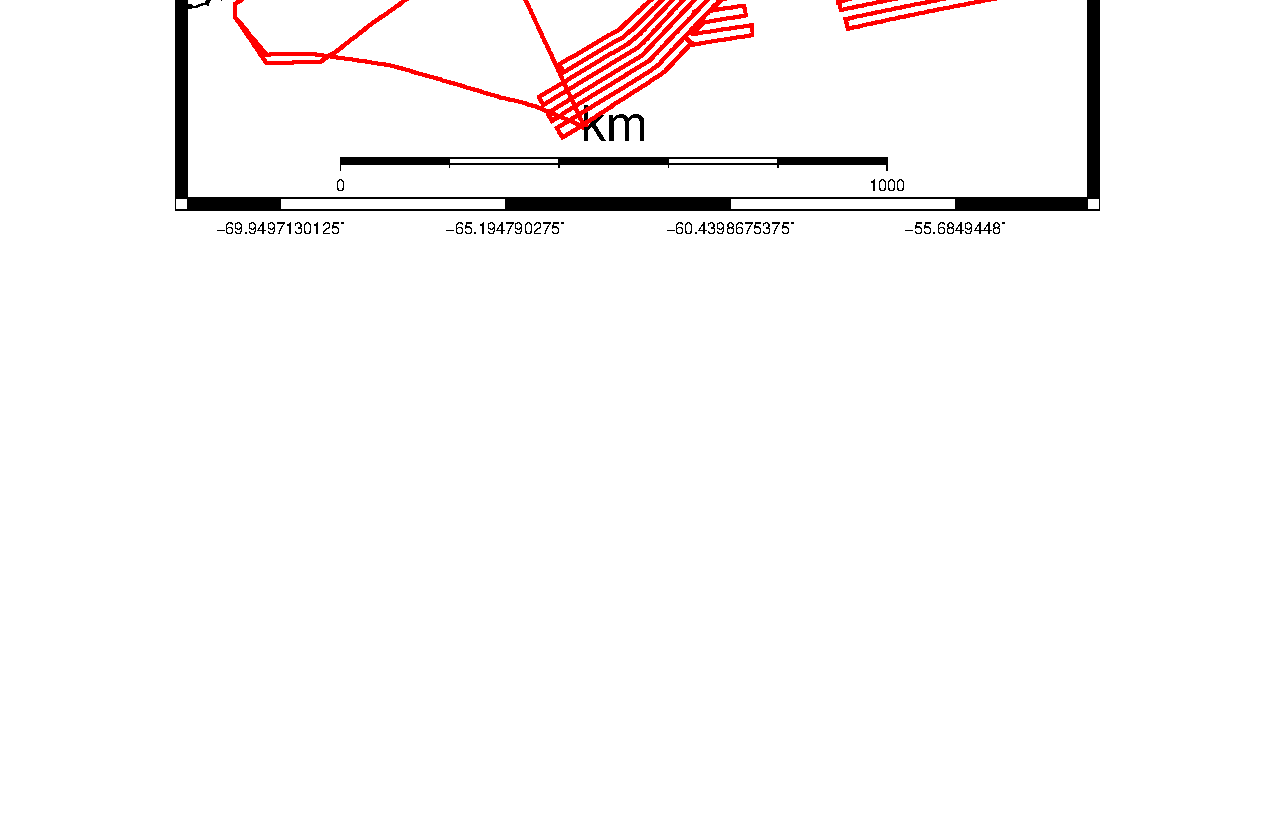
\includegraphics[width=1.2\textwidth]{AT22_control_track.pdf}
%		\end{tabular}
%		\end{figure}
		
	\newpage	
	\section{Creating a Custom Parser}
	\label{custom_parser}
		\subsection{Requirements of your dataset}
		
NavManager requires dates, timestamps, latitudes, and longitudes for every data point.  If you are setting up a navigation system and are looking for formatting guidance, see section \ref{best_practices} for formatting best practice guidelines.  Because not all systems record inertial data, NavManager does not rely on this for velocity and acceleration values.
		
		\subsection{Required additions to the code}
		
There are two locations where parsing code needs to be added in order for navcopy.php to successfully convert data to the r2rnav format.  The first step in parsing the data is the creation of a time ordered list of the raw data files.  This is done with a function called navdatalist.  The next step is to copy the data specified by navdatalist into the r2rnav format.  This is done with the navcopy function.

The navdatalist function can be found in the file include/navdatalist.inc.php.  Add a case for your file format in the main switch statement of the function.  During this step, only temporal information needs to be parsed.

The navcopy function can be found in the file include/navcopy.inc.php.  Again, a case for your file format name needs to be added to the main switch statement of the function.  Both temporal and spatial information need to be parsed into the r2rnav format.

		\subsection{Existing resources}
		
If your data contains some form of a NMEA 0183 string, many tools exist within NavManager for you to draw upon.  Check out the file include/nmeatools.inc.php.  Here you can find classes and functions for parsing NMEA strings.  Example usage can be found by digging through navcopy.inc.php and seeing how other formats are parsed.
	
	\newpage		
	\section{Troubleshooting}
	\label{troubleshooting}
		
		\subsection{Percent completeness errors}
		\label{percent_completeness_errors}
Percent completeness problems usually occur because of varying sampling rates.  Check STDOUT to make sure that the mode value for epoch interval is the primary mode.  If there is more than one mode for interval, the percent completeness cannot be determined - and probably came out to be greater than 100.
	
Percent completeness is intended to give quality information on a dataset with a constant epoch interval.  If data does not have a constant sampling rate the percent completeness record should be discarded so as not to be misinterpreted.
	
		\subsection{Data gaps}
		\label{data_gaps}
Large gaps in data could be real or they could be a indicator of a problem with data files being mis-ordered by navcopy.php.  First check the data (or metadata) for evidence of a real gap in the data.  Ideally navigation system should not be turned off during an expedition, but sometimes this happens.
	
If navcopy.php is not ordering your navigation files correctly, this might be due to files beginning with nonsense date values.  Look for incomplete lines at the beginning or end of files.  Mis-ordering of files can also because by location records being out of sequence.

	\newpage
	\section{References}
		\subsection{The r2rnav Format}
		\label{r2rnav_spec}

\begin{lstlisting}
http://get.rvdata.us/format/100002/format-r2rnav.txt
\end{lstlisting}
		
		\subsection{NMEA Strings}
		\label{nmea_spec}
		
\begin{lstlisting}
http://www.agt.bme.hu/tantargyak/bsc/bmeeoafav49/NMEAdescription_gy_12.pdf
\end{lstlisting}
		
		\subsection{Format Best Practices}
		\label{best_practices}
		
\begin{lstlisting}
http://www.rvdata.us/system/files/private/
	Recommended-Best-Practices-for-Navigation-Data-Collection.pdf
\end{lstlisting}

		\subsection{Generic Mapping Tools (GMT)}
		\label{GMT}
		
\begin{lstlisting}
http://gmt.soest.hawaii.edu/
\end{lstlisting}

		
\end{document}
